\documentclass[12pt,letterpaper]{hmcpset}
\usepackage[margin=1in]{geometry}
\usepackage{graphicx}
\usepackage{amsmath}
\usepackage{multirow}

% info for header block in upper right hand corner
\name{}
\class{Math 35 - Section }
\assignment{Homework 3}
\duedate{Tuesday, November 10, 2015}

\newcommand{\pn}[1]{\left( #1 \right)}
\newcommand{\abs}[1]{\left| #1 \right|}
\newcommand{\bk}[1]{\left[ #1 \right]}
\newcommand{\vc}[1]{\left\langle #1 \right\rangle}

\newcommand{\pder}[2]{\frac{\partial #1}{\partial #2}}

\newcommand{\fx}{f \left( x \right) =}
\newcommand*\LH{\ensuremath{\overset{\kern2pt L'H}{=}}}

\begin{document}

\problemlist{3.\{1.9, 1.15, 2.15, 2.17, 2.18, 2.32, 2.33\}, 4.\{1.5, 2.13, 3.28.\{abc\}, 3.29.\{abc\}, 3.30.\{abc\}, 31, 35\}}

% 3.1.9 %
\begin{problem}[3.1.9]
An individual named Claudius is located at the point 0 in the accompanying diagram.\\
\begin{center}
	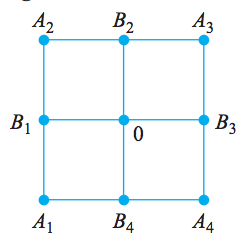
\includegraphics{Nov_10_1.png}
\end{center}
Using an appropriate randomization device (such as a tetrahedral die, one having four sides), Claudius first move to one of the four locations $B_1$, $B_2$, $B_3$, $B_4$. Once at one of these locations, another randomization device is used to decide whether Claudius next returns to 0 or next visits one of the other two adjacent points. This process then continues; after each moe, another move to one of the (new) adjacent points is determined by tossing an appropriate die or coin.\\
\\(a) Let $X$ = the number of moves that Claudius makes before first returning to 0. What are possible values of $X$? Is $X$ discrete or continuous?\\
\\(b) If moves are allowed also along the diagonal paths connecting 0 to $A_1$, $A_2$, $A_3$, and $A_4$, respectively answer the questions in part (a).
\end{problem}

\begin{solution}

\end{solution}
\newpage



% 3.2.15 %
\begin{problem}[3.2.15]

Many manufacturers have quality control programs that include
inspection of incoming materials for defects. Suppose
a computer manufacturer receives computer boards in
lots of five. Two boards are selected from each lot for
inspection. We can represent possible outcomes of the selection
process by pairs. For example, the pair (1, 2) represents
the selection of boards 1 and 2 for inspection.\\
\\(a) List the ten different possible outcomes.\\
\\(b) Suppose that boards 1 and 2 are the only defective
boards in a lot of five. Two boards are to be chosen at
random. Define $X$ to be the number of defective boards
observed among those inspected. Find the probability
distribution of $X$.\\
\\(c) Let $F(x)$ denote the cdf of $X$. First determine $F(0) = P(X \leq 0)$
, $F(1)$, and $F(2)$; then obtain $F(x)$ for all other $x$.
\end{problem}

\begin{solution}

\end{solution}
\newpage

% 3.2.17 %
\begin{problem}[3.2.17]
A new battery?s voltage may be acceptable $(A)$ or unacceptable
$(U)$. A certain flashlight requires two batteries, so batteries
will be independently selected and tested until two
acceptable ones have been found. Suppose that 90$\%$ of all
batteries have acceptable voltages. Let $Y$ denote the number
of batteries that must be tested.\\
\\(a) What is $p(2)$, that is, $P(Y = 2)$?\\
\\(b) What is $p(3)$? [\textit{Hint}: There are two different outcomes
that result in $Y = 3$.]\\
\\(c) To have $Y = 5$, what must be true of the fifth battery
selected? List the four outcomes for which $Y = 5$ and
then determine $p(5)$.\\
\\(d) Use the pattern in your answers for parts (a)?(c) to obtain
a general formula for $p(y)$.
\end{problem}

\begin{solution}

\end{solution}
\newpage
% 3.2.18 %
\begin{problem}[3.2.18]
8. Two fair six-sided dice are tossed independently. Let $M$ = the maximum
of the two tosses (so $M(1,5) = 5$, $M(3,3) = 3$, etc.).\\
\\(a) What is the pmf of $M$? [\textit{Hint}: First determine $p(1)$, then
$p(2)$, and so on.]\\
\\(b) Determine the cdf of $M$ and graph it.

\end{problem}

\begin{solution}

\end{solution}
\newpage

% 3.3.32 %
\begin{problem}[3.3.32]
An appliance dealer sells three different models of upright
freezers having 13.5, 15.9, and 19.1 cubic feet of storage
space, respectively. Let $X$ = the amount of storage space
purchased by the next customer to buy a freezer. Suppose
that $X$ has pmf
\begin{center}
	\begin{tabular}{c|c c c}
		 x & 13.5 & 15.9 & 19.1\\
 		\hline
 		p(x) & 0.2 & 0.5 & 0.3 \\
	 \end{tabular}
\end{center}
(a) Compute $E(X)$, $E(X^2$), and $V(X)$.\\
\\(b) If the price of a freezer having capacity $X$ cubic feet is$25X - 8.5$, what is the expected price paid by the next
customer to buy a freezer?\\
\\(c) What is the variance of the price $25X - 8.5$ paid by the
next customer?\\
\\(d) Suppose that although the rated capacity of a freezer is $X$, the actual capacity is $h(X) = X - .01X^2$. What is the expected actual capacity of the freezer purchased by the
next customer?
\end{problem}

\begin{solution}

\end{solution}
\newpage
% 3.3.33 %
\begin{problem}[3.3.33]
Let $X$ be a Bernoulli rv with pmf as in Example 3.18.\\
\\(a) Compute $E(X^2)$.\\
\\(b) Show that $V(X) = p(1-p)$.\\
\\(c) Compute $E(X^{79})$.
\end{problem}

\begin{solution}

\end{solution}
\newpage
% 4.1.5 %
\begin{problem}[4.1.5]
A college professor never finishes his lecture before the end of
the hour and always finishes his lectures within 2 min after the
hour. Let $X$ = the time that elapses between the end of the
hour and the end of the lecture and suppose the pdf of $X$ is
\begin{center}
$f(x) = \begin{cases}
	kx^2 & 0 \leq x \leq 2 \\
	0 & \mbox{otherwise}
	\end{cases}$
\end{center}
(a) Find the value of $k$ and draw the corresponding density
curve. [\textit{Hint}: Total area under the graph of $f(x)$ is 1.]\\
\\(b) What is the probability that the lecture ends within 1 min
of the end of the hour?\\
\\(c) What is the probability that the lecture continues beyond
the hour for between 60 and 90 sec?\\
\\(d) What is the probability that the lecture continues for at
least 90 sec beyond the end of the hour?
\end{problem}

\begin{solution}

\end{solution}
\newpage

% 4.2.13 %
\begin{problem}[4.2.13]
Example 4.5 introduced the concept of time headway in
traffic flow and proposed a particular distribution for $X$ = 
the headway between two randomly selected consecutive
cars (sec). Suppose that in a different traffic environment,
the distribution of time headway has the form
\begin{center}
$F(x) = \begin{cases}
	\qquad 0 & x \leq 0 \\
	\dfrac{x}{4}\Big[1 + \ln{\dfrac{4}{x}}\Big] & 0 < x \leq 4\\
	\qquad1 & x >4
	\end{cases}$
\end{center}
(a) Determine the value of $k$ for which $f(x)$ is a legitimate pdf.\\
\\(b) Obtain the cumulative distribution function.\\
\\(c) Use the cdf from (b) to determine the probability that
headway exceeds 2 sec and also the probability that
headway is between 2 and 3 sec.\\
\\(d) Obtain the mean value of headway and the standard
deviation of headway.\\
\\(e) What is the probability that headway is within 1 standard
deviation of the mean value?
\end{problem}

\begin{solution}

\end{solution}
\newpage

% 4.3.28 %
\begin{problem}[4.3.28]
Let $Z$ be a standard normal random variable and calculate
the following probabilities, drawing pictures wherever
appropriate.\\
\\(a) $P(0 \leq Z \leq 2.17)$
\\(b) $P(0 \leq Z \leq 1)$
\\(c) $P(-2.50 \leq Z \leq 0)$

\end{problem}

\begin{solution}

\end{solution}
\newpage

% 4.3.29 %
\begin{problem}[4.3.29]
In each case, determine the value of the constant $c$ that
makes the probability statement correct.\\
\\(a) $\Phi(c) = .9839$
\\(b) $P(0 \leq Z c) = .291$
\\(c) $P(c \leq Z) = .121$

\end{problem}

\newpage

% 4.3.30 %
\begin{problem}[4.3.30]
Find the following percentiles for the standard normal distribution.
Interpolate where appropriate.\\
\\(a) 91st
\\(b) 9th
\\(c) 75th

\end{problem}

\begin{solution}

\end{solution}
\newpage

% 4.3.31 %
\begin{problem}[4.3.31]
Determine $z_\alpha$ for the following:\\
\\(a) $\alpha = 0.0055$
\\(b) $\alpha = 0.09$
\\(c) $\alpha = 0.663$

\end{problem}

\begin{solution}

\end{solution}
\newpage
% 4.3.35 %
\begin{problem}[4.3.35]
Suppose the diameter at breast height (in.) of trees of a
certain type is normally distributed with $\mu = 8.8$ and $\sigma = 2.8$
, as suggested in the article ?Simulating a
Harvester-Forwarder Softwood Thinning? (\textit{Forest
Products J.}, May 1997: 36?41).\\
\\(a) What is the probability that the diameter of a randomly
selected tree will be at least 10 in.? Will exceed
10 in.?\\
\\(b) What is the probability that the diameter of a randomly
selected tree will exceed 20 in.?\\
\\(c) What is the probability that the diameter of a randomly
selected tree will be between 5 and 10 in.?\\
\\(d) What value $c$ is such that the interval
includes 98$\%$ of all diameter values?\\
\\(e) If four trees are independently selected, what is the
probability that at least one has a diameter exceeding
10 in.?
\end{problem}

\begin{solution}

\end{solution}
\newpage

\end{document}
